\section{ReiserFS}
\subsection{Introducción}
\begin{frame}{Introducción}
  \begin{itemize}
    \item Sistema de proposito general.
    \item Muy bueno en tratamiento de ficheros pequeños.
    \item Primero sistema de ficheros con Journaling incluido en el kernel de Linux.
    \item Es el sistema de ficheros por defecto en varias distribuciones.
    \item Actualmente Namesys ha dejado el desarrollo de ReiserFS para centrarse en su sucesor Reiser4.
  \end{itemize}
\end{frame}

\subsection{Caracteristicas}
\begin{frame}{Caracteristicas}
  \begin{itemize}
    \item Journaling
    \item ACLs
    \item Permisos POSIX
    \item Tamaño maximo: 16TB
    \item Tamaño maximo de fichero: 16TB
    \item Maximo de caracteres de nombre de fichero: 256B
    \item Maximo numero de ficheros: 4.294.967.293
  \end{itemize}
\end{frame}

\subsection{Estructura}
\begin{frame}{Estructura}
  \begin{itemize}
    \item Al principio de la particion nos encontramos el sector de arranque.
    \item Justo despues se encuentra el superblock.
    \item Para el resto de la particion se van alternando mapas de bits de bloques y bloques de datos.
    \item Cada mapa de bits de bloques se refiere al bloque de datos que queda despues de el y nos da informacion sobre los bloques libres  y ocupados.
    \item Cada bloque de datos contiene los datos e inodos.
  \end{itemize}
\end{frame}

\begin{frame}{Estructura}
  \begin{center}
    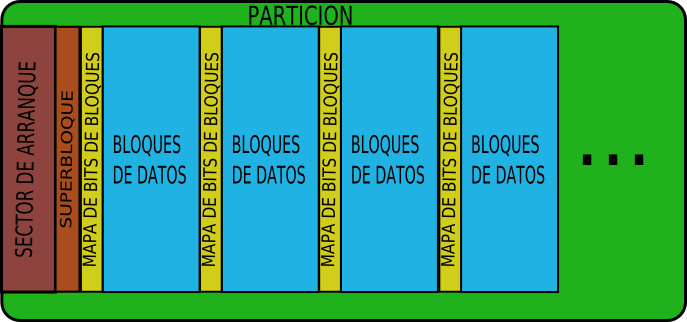
\includegraphics[height=5.5cm]{imgs/reiserfs_struct.png}
  \end{center}
\end{frame}

\begin{frame}{Ficheros}
  \begin{itemize}
    \item Existen 4 tipos de objetos: stat, directorios, directos e indirectos.
    \item Todos los ficheros en reiser tienen asociado un objeto stat, el cual almacena informacion de permisos.
    \item Los directorios a su vez tienen asociados uno o mas objetos del tipo directorio, tantos como hagan falta para almacenar todas las entradas del directorio.
    \item Los ficheros regulares, si son pequeños se asocian a un objeto directo que almacena los datos, si son grandes se asocia a uno o varios objetos indirectos que contienen punteros a bloques de datos.
  \end{itemize}
\end{frame}

\begin{frame}{Ficheros}
  \begin{center}
    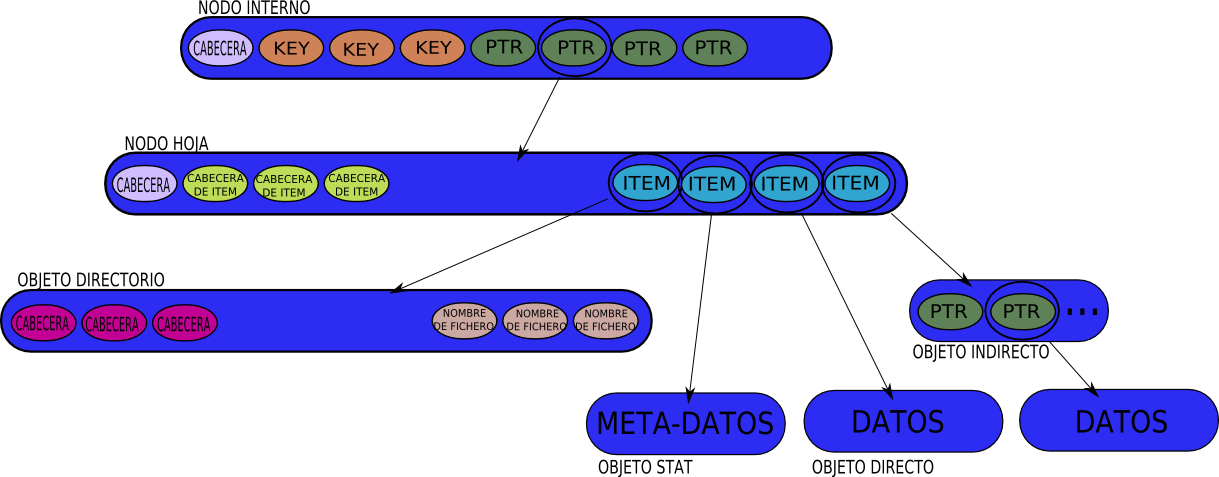
\includegraphics[height=4.5cm]{imgs/reiserfs_files.png}
  \end{center}
\end{frame}
